\chapter{Introduction}
The course Experts in Teamwork (EiT) is designed to give students experience with cross disciplinary projects to enhance their communication and collaborative abilities, preparing them for the challenges they will meet in their future work environments~\cite{ntnu_what_is_eit}. 

We took part in the village “Virtual and Augmented Reality for Games, Health and Education” which focuses on the exciting new possibilities of virtual and augmented reality. As this is a young field we were given the opportunity to experiment with different ideas, with the potential of shaping the future of virtual reality (VR) and augmented reality (AR). 

Our project, Conductor Hero, is a VR rhythm game that introduces the player to the world of ensemble conducting. The project was an exciting first hand-experience of the challenges faced in virtual reality, and also presented us with the requirements of working in a cross disciplinary team. This document will give the reader an overview over the situations, reflections and experiences we encountered throughout the semester.


\section{Group formation}
\subsection{Animal Model}
The 6-animal model, developed by Simon McCallum~\cite{six_animal_model}, focus on the different roles of group members. The model uses six animal avatars (bear, wolf, cat, puppy, owl, and rabbit) to represent the different roles, creating a cognitive distance between the role and the individual, helping with group organisation and communication. The bear is the group leader, while the wolf is the manager ensuring that everyone in the group is participating. The cat takes on the role of the critic, looking for flaws in proposed ideas, with the puppy being the complete opposite, enthusiastic and supporting of every idea. The owl has the role of the processor and ensures that objectives are met, and finally the rabbit acts as a facilitator, volunteering to get coffee or other resources needed by the group. In this model every animal is considered equally important for group success.

During the first village day the each student was encouraged to identify themselves with one of the 6 animals. The people who identified as bears were told to stand up, and the others were told to form groups with the different bears. These groups should ideally have a good mix of the different animals. Through this exercise we ended up with our group, consisting of
Per-Morten (bear), Andreas (owl), Yijie (puppy), Rikhart (cat), Sabina (rabbit), and Ellinor (wolf). 


\subsection{Assigning roles} \label{sec:assigning_roles}
After forming groups based on the 6-animals model, we performed a triangle exercise. An image from the exercise can be seen in Figure~\ref{fig:triangle_exercise}. Here, each group member were given the chance to inform the others what they could bring to the project, in terms of personality,  practical experiences and theoretical knowledge. An overview of the skills can be seen in Table~\ref{table:skills}

\begin{figure}[h]
    \centering
    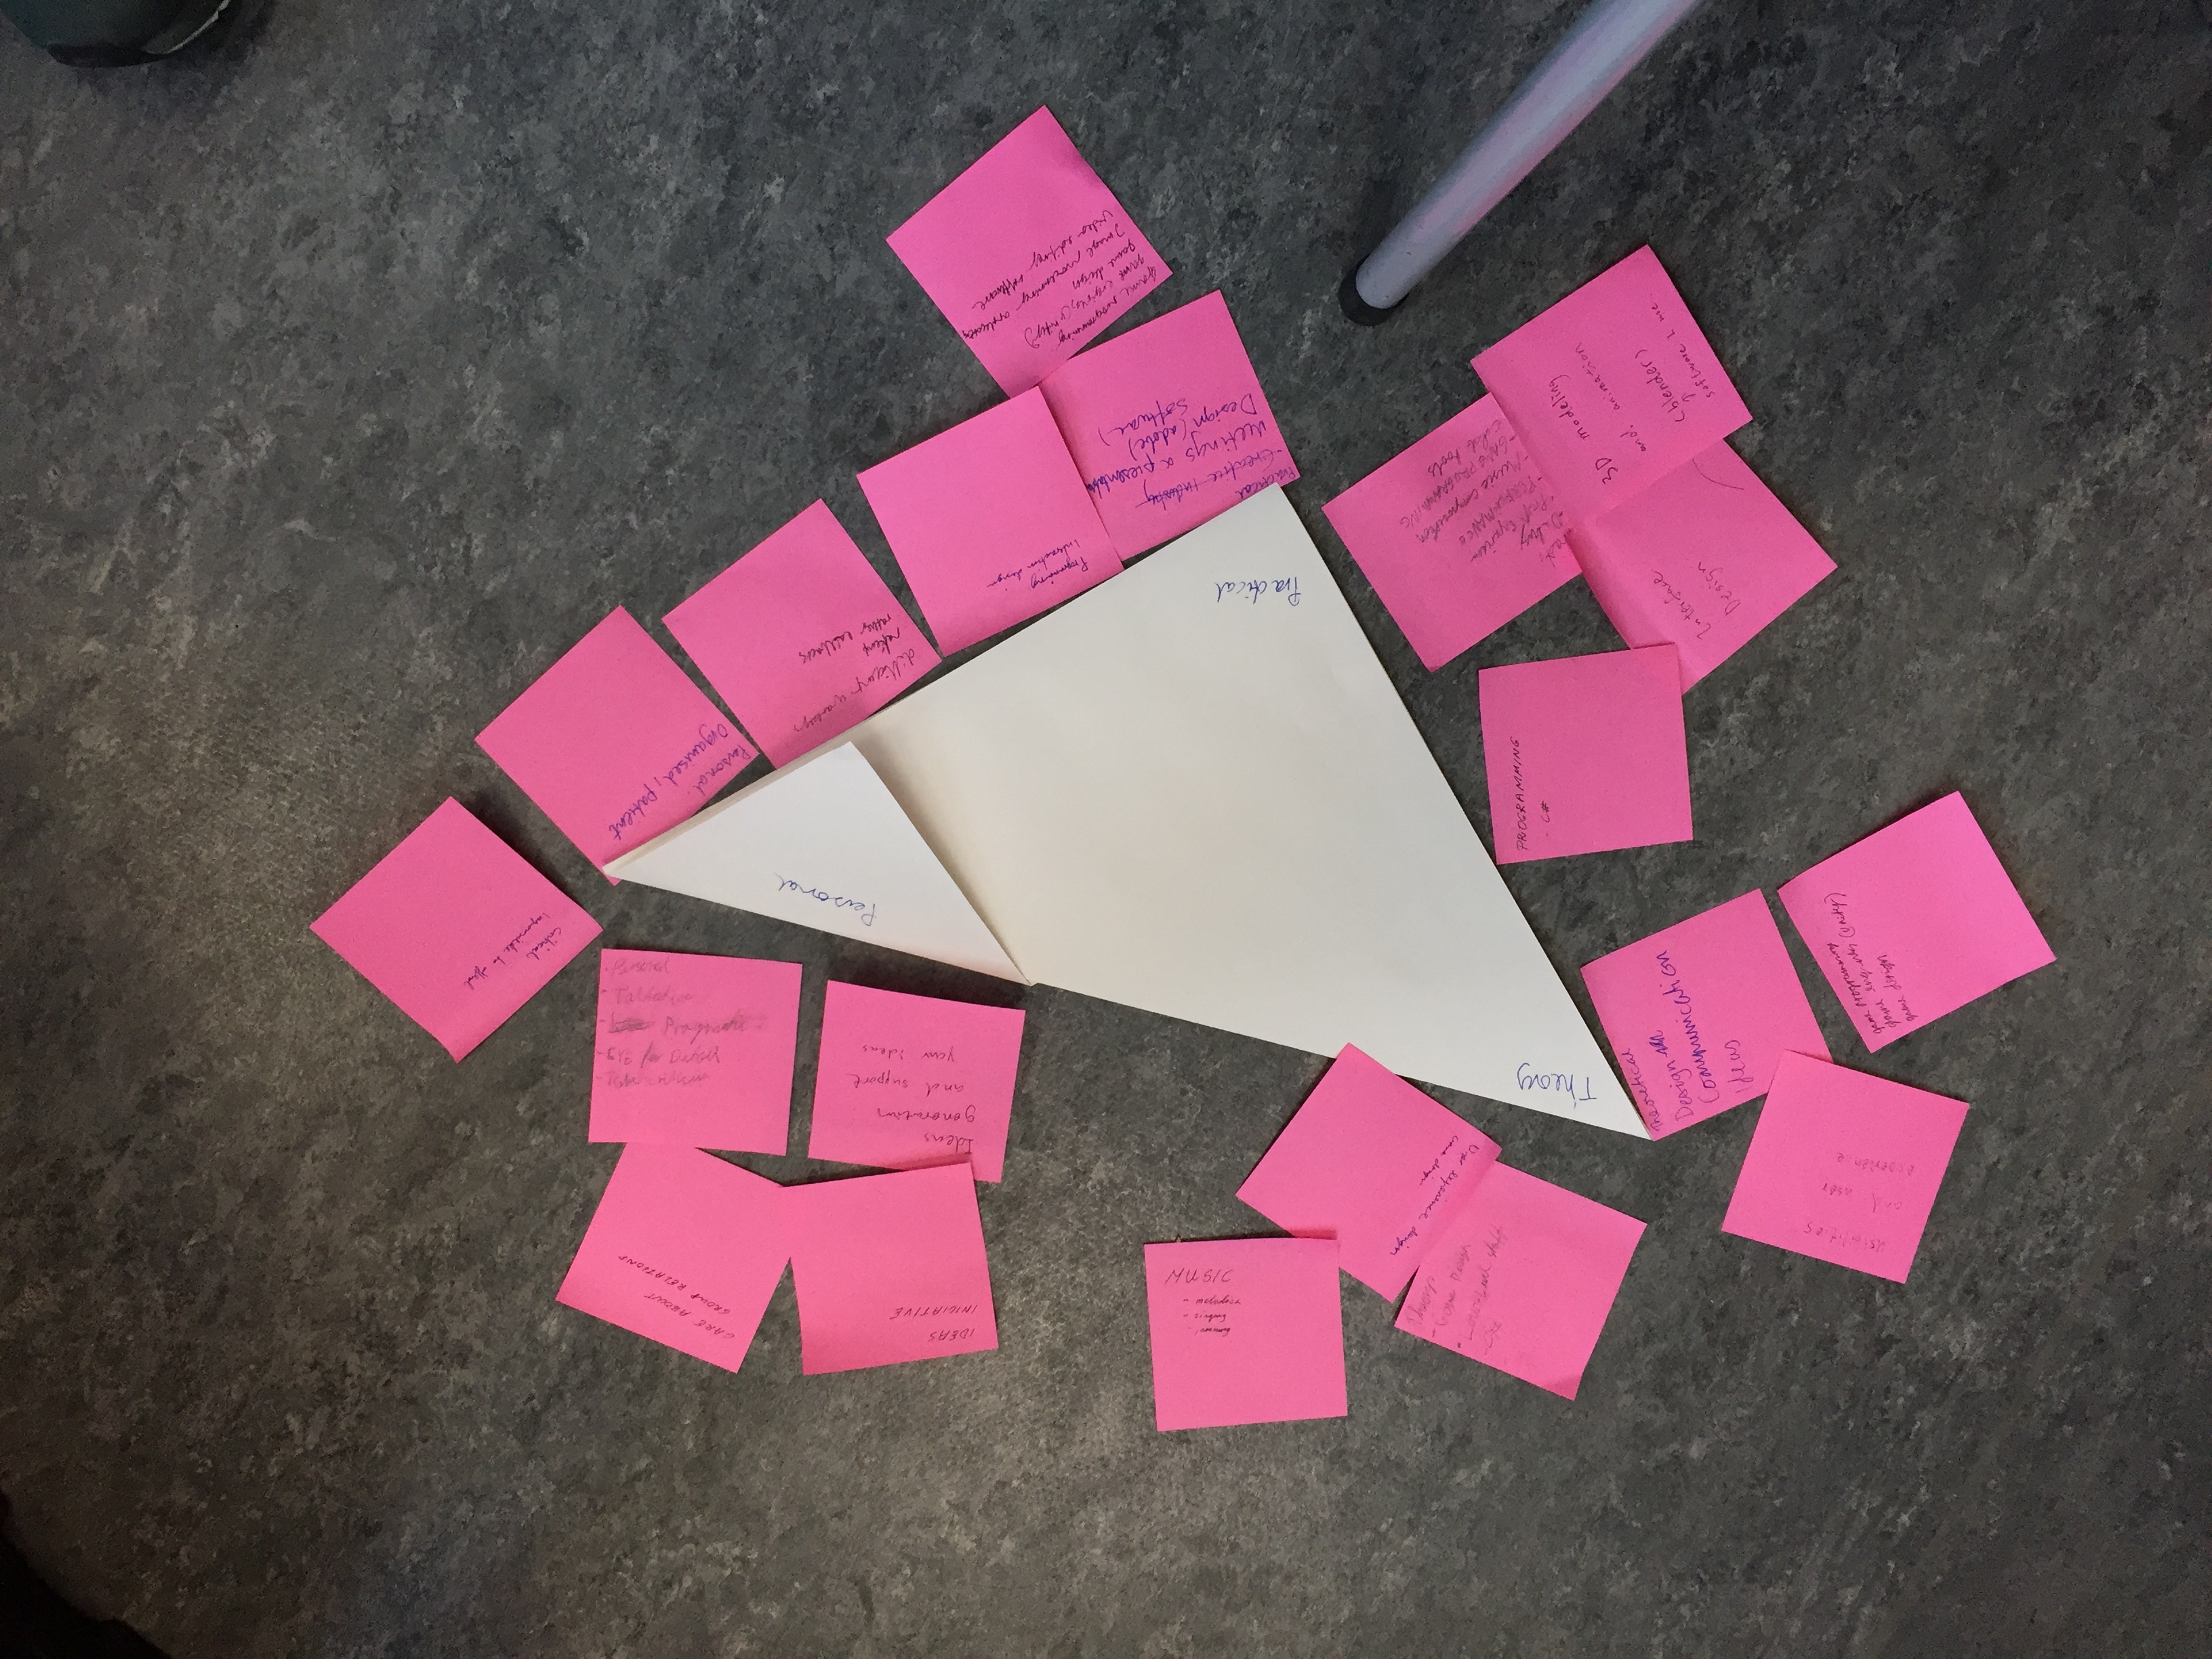
\includegraphics[width=0.9\textwidth]{images/triangle_exercise}
    \caption[Exercise for surveying skills within the group.]{Exercise for surveying skills within the group. Each triangle corner: the type of value. Post its: the values team members contribute to the group. The exercise depicted formed the basis for the table below.}
    \label{fig:triangle_exercise}
\end{figure}

\begin{table}[H]
    \centering
    \begin{tabularx}{\linewidth}{ | l | X | X |}
        \hline
        \textbf{Member} & \textbf{Skill} & \textbf{Background}  \\
        \hline
        Rikhart & Design, Programming, Critical thinking & Web Development, Interaction Design \\
        \hline
        Sabina & Design, Programming, Music & Web application development, Interaction Design \\
        \hline
        Per-Morten & Programming, Music Composing & Game Programming, International Marketing \\ 
        \hline
        Andreas & Programming, Experience with the Unity Engine, Music & Game Programming  \\
        \hline
        Yijie & Design, 3D modelling, animation & Digital Media, Interaction Design \\
        \hline
        Ellinor & Design, Graphics design, Music & Graphic Design, Art direction, Interaction Design  \\
        \hline
    \end{tabularx}
    \caption{Table of the groups skillset.}
    \label{table:skills}
\end{table}

After performing the exercise, we had a better awareness of each others personalities and skills, and established more specific roles for our group. Ellinor took the role of project lead, as she was interested in exploring her leadership potential, and Per-Morten was happy to pass on the role. Yijie, had experience with 3D modeling and animation and therefore took the role of art director. Per-Morten, who had a strong leadership skill and an interest in software architecture took the role of technical lead. Andreas took the role of Unity expert as he had the most experience with the Unity game engine. He was also given the responsibility of taking notes to record the process and progress of the group. As Sabina and Rikhart had backgrounds in both development and design it was decided that they should work as bridges between the designers and programmers. Additionally, Rikhart was delegated the role of UI expert, based on his previous experience within the field. Sabina volunteered to take the role of public relationship manager, as we intended to contact several external professionals.
% TODO: UPDATE after changes are done
\section{Group Members}
\begin{figure}[tpbh]
    \centering
    \includegraphics[width=0.9\textwidth]{images/Conductor_team}
    \caption[Group Photo]{Our group, 24 eyes}
    \label{fig:conductor_team}
\end{figure}
Below follows a more in-depth overview of the group members (shown in Figure~\ref{fig:conductor_team}), and our thoughts going into the project.
\subsection{Rikhart Vigdal Bekkevold}
\textbf{Nationality:} Norwegian \\
\textbf{Study:} Master in Interaction Design \\
\textbf{Background:} Web Development, Interaction Design \\
\textbf{Role:} Cross-discipline communication, UI expert

Entering this project I already knew that I was a very critical person. I have always seen this as a benefit when it comes to seeing the holes in ideas and in identifying problems. I have also experienced that it can be a less positive thing if it is dominating, hindering progress and creating conflicts in groups I have partaken in. Knowing this in advance, it was something I tried to work on, and to make sure it didn’t become too dominating in our groupwork. Before this course I had been in many different groups, ranging in success from bad to decent, but never good. Because of this, group work had always been a chore to me.


\subsection{Sabina Niewiadomska}
\textbf{Nationality:} Polish \\
\textbf{Study:} Master in Applied Computer Science \\
\textbf{Background:} Web application development, Interaction Design \\
\textbf{Role:} Cross-discipline communication, Public relations

I joined the EiT course with both experiences from students projects and work. In students projects, it often happened that I become a leader, students with which I was cooperating were describing me as "person bringing initiative" or "good coordinator". In the real work environment, I've never had a  chance to become a team leader.In the first classes, we were asked to represent ourselves as a type of animal. Knowing my duties this semester I decided that I would like to take a role of a wolf or an owl. Some people were suggesting that I would be a good wolf (good work coordinator) and some that I would be a good owl (I like to organize group work with tools like Microsoft Planner/Trello/SharePoint ). Unfortunately, when I joined this group the positions of wolf or owl were already taken, but it wasn't a problem for me. As a result, I was assigned the rabbit role. Before EiT course I was totally unfamiliar with Virtual and Augmented Reality products and development process. I don't play any games regularly. My programming skills are strong in rapid software development in ASP.NET for financial applications (both desktop and web solutions, but mostly web development). I also have a good understanding of databases problems and a strong interest in User Experience issues. One of the biggest challenges of this project was to learn the concept of game programming and Unity for Virtual and Augmented Reality.

\subsection{Per-Morten Straume}
\textbf{Nationality:} Norwegian \\
\textbf{Study:} Master in Applied Computer Science \\ 
\textbf{Background:} Game Programming, International Marketing \\
\textbf{Role:} Chief Technical Officer

Before taking the course I already had a fair amount of group experience, both mono-discipline and cross-discipline projects, in professional and academic settings. Because of this I already had some ideas of my behavior in groups, and how it affected group dynamics. I was aware that I can be dominating in group, and also that I can be quite vocal and honest about my views. However, I always try to be open to others views, and promoting discussions to reach optimal solutions to problems. My wish for the course was that if I was completely wrong about my theories of myself in group dynamics I would be made aware of them.

Throughout my higher education I usually ended up being the leader in group projects, mainly because no one else wanted to. However, I have never been really comfortable with this role, and decided for this project that I did not want to be project lead. One of the reasons for this is that I often struggle with several managerial tasks like structuring and planning because of my ADHD diagnosis. Nonetheless, I did volunteer to be a bear on the first village day, as there were not that many students who seemed interested in the role.


\subsection{Ida Ellinor Syverinsen}
\textbf{Nationality:} Norwegian \\
\textbf{Study:} Master in Interaction Design \\
\textbf{Background:} Graphics Design, Art Direction, Interaction Design \\
\textbf{Role:} Chief Executive Officer

At the beginning of the course I decided to keep an open mind to the project, even though I had heard mixed, and often negative, opinions about the course from other students. During the group formation, I picked “wolf” as my primary animal character, with “cat” as a second option. I found this fitting as I am not afraid of voicing my opinion, and can sometimes enjoy playing “Devil’s advocate”. I decided to try to join a group where I had not previously worked with any of the other group members, which I managed to. 

I already had a lot of experience working in groups before starting this project, both from educational and professional settings. This also includes the first half of my master programme, in which all courses have included group projects. My experiences with group projects have mostly been positive since commencing higher education, and I consider myself to be well versed in teamwork. I am, however, also aware that I am a typical “introvert”, meaning that working with, and also spending time with, others can sometimes make me feel more tired and “drained” than working individually. 


\subsection{Andreas Wang}
\textbf{Nationality:} Norwegian \\
\textbf{Study:} Master in Applied Computer Science \\
\textbf{Background:} Game Programming \\ 
\textbf{Role:} Unity Engine Expert

Prior to entering the project I already had a fair amount of experience working in various groups. Some of these were relatively well performing while some also were dysfunctional. I already knew the importance of teamwork for larger projects due it being central for game programmers. It was exciting to hear that we were going to work on VR/AR applications in this course and I was interested in seeing how cooperating across disciplines would work as this is something that has not been a part of my previous education. 

\subsection{Yijie Zhou}
\textbf{Nationality:} Chinese \\
\textbf{Study:} Master in Interaction Design \\
\textbf{Background:} Digital Media, Interaction Design \\
\textbf{Role:} Art Director

Before the EIT course, I have gotten used to working in multidisciplinary teams both for school projects and in the real working environment, though I never pay attention to the team, theories about teamwork, or my role in the team. During my previous projects and working experience, I used to think that maintaining the team was not my responsibility and just focused on my own work. For conflicts I encountered, I usually just let them go and didn’t try to handle them properly. Generally, I cared more about my personal work than the group work. This made me less active during the group discussion and I sometimes lost the big picture of the group work. I was aware that though I was always willing to contribute to the group and try my best to accomplish my tasks, ignoring the group is definitely harmful both for myself and the group. I hope that during this course, I could improve the defects mentioned above and focus more on the group. Additionally, I hope to be able to have more opinion exchanges with other group members and contribute ideas more actively. 
 